\chapter{Dynamic Queries} \label{ch:dynamicQueries}
% structure of this chapter:
% main = dynamic queries
% Explain:
% - what I mean by that
% - basic requirements = viewer
% - beauty = can be extendend, 
%   more filetypes, not only geometry
% - 3 possible implementations, 
%   computation always in different place
% - making use of EXISTING DATA,
%   can be extended to new dedicated ontologies
This chapter introduces the concept of dynamic querying. In this thesis, it refers to the automatic generation of queries responsible for obtaining the data needed to visualize building elements from a \ac{bim} model within an \ac{rdf} graph. The examples are presented as static SPARQL queries, since the automation itself depends on the implementation or framework used. A link to the appendix is provided, where the implementation within the prototype of this thesis is explained.

The structure is as follows: first, the requirements for the viewer are researched, as its functioning will dictate the output of the queries. Second, the capabilities of the viewer are explored in relation to the visualization of semantic data, thus emphasizing the added value of working with Linked Data. Third, three types of dynamic queries for culling are presented, each with its own advantages and disadvantages.

% - importance of viewer
% - refer to state of the art existing viewers
\section{Requirements} \label{sec:viewerRequirements}
% - different file formats, different sources.
% - reusing first diagram
% - why XEOKIT sdk (practical)
A viewer designed to visualize data stored in an \ac{rdf} graph is required to understand the data stored within it. Therefore, the requirements for the viewer align with those of its source, the \ac{rdf} graph. Section \ref{sec:fog}, which discusses the use of both the \ac{fog} and \ac{omg} ontologies, offers an overview of the available options in terms of file format and file source. The \ac{fog} ontology supports the description of a wide range of geometry formats, as illustrated in Table \ref{tab:geometryFormats}. In conjunction with the \ac{omg} ontology, which allows for the description of the file source using the datatype of the literal, it can be concluded that the viewer should be able to handle a broad spectrum of file formats, preferably described in the \ac{fog} ontology, and accept both remote files and literal values.

\begin{table}[H]
    \centering
    \begin{tabular}{llll}
        \toprule
        COLLADA & Compressed LAS  & Compressed Nexus      & DWG      \\
        E57     & GeoJSON         & Well Known Text SFA   & GML      \\
        IFC     & IGES            & LAS Point Cloud       & Nexus    \\
        OBJ     & PCD Point Cloud & Uncompressed LAS      & Revit    \\
        Rhino   & Shapefile       & Simple Feature Access & SketchUp \\
        SPFF    & STEP SPFF       & Uncompressed Nexus    & SVG      \\
        PLY     & STL             & Well Known Binary SFA & X3D      \\
        glTF    &                 &                       &          \\ \bottomrule
    \end{tabular}
    \caption[\acs{fog} ontology geometry formats]{List of geometry formats that can be assigned with the \acs{fog} ontology.\footnotemark}
    \label{tab:geometryFormats}
\end{table}
\footnotetext{\cite{fog}}

\section{Beyond geometry}
% - possibilities of viewer extends classical approach
This section highlights the adavantages a viewer based on Linked Data has over a viewer based on traditional file-based systems, by extenting the thought of a 3D viewer to its ability to visualise non geometric data from its source. \ac{ldbim} links geometrical entities to their corresponding semantic data, which can be visualised in the viewer. This allows for the visualisation of data that is not directly related to the geometry of the building elements, such as the physical properties of a wall or the cost of a door. The possibilities are endless, as long as the data is available in the \ac{rdf} graph. The following sections will discuss different possible implementations.


\subsection{\acs{bcf} integration} \label{sec:bcf}
% - BCF viewpoints in xeokit
% - what is bcf...
As a first possible implementation of non-geometric data, this section examines the \ac{bcf} buildingSMART standard. \ac{bcf} is an open file format that enables the creation and communication of issues about \ac{bim} models \footcite{bcf}. Both it and its translation in the Semantic Web as \ac{bcfowl} \parencite{bcfOWL} link a screenshot, a camera angle, and a list of concerned entities to form a specific issue \footcite{bcfCollab}.

This type of semantic offers two types of implementations. The first is the positioning of a screenshot, together with its camera position and orientation, within the 3D scene. This allows for the visualization of issues, which can be linked to the screenshot, in the viewer, offering communication integration. The second implementation involves the metadata surrounding issues that can be used as visual properties to feed specific queries. This type of implementation is discussed in the next section, \nameref{sec:visualSemantic}.

\subsection{Visualising semantic} \label{sec:visualSemantic}
% - element associated data
% - physical: thermal, acoustic, ...
% - non-physical: cost, time, pothologies, ...
% - all  with temporal dimension / history
When examining semantics such as physical properties of entities, free from geometric and spatial data (see \nameref{sec:bcf}), a visual interpretation superimposed on the viewer offers powerful rendering possibilities. By coloring elements based on their properties, both physical and non-physical, the viewer can be used to detect anomalies or insights in the model, in a feature-rich output medium.

Physical properties such as thermal, acoustic, structural, and others, or non-physical properties like cost, time, and pathologies, can all be described and linked in the \ac{rdf} graph. The expressive capabilities of \ac{sparql} enable complex and fine-grained queries, offering application-specific query creation about these properties. By selecting a specific subset or combining them, a user or developer can transform the viewer into a powerful tool.

As such, the viewer is expected to comply with a multitude of requirements, which are not all covered in this thesis. Chapter \nameref{ch:modularApproach} thus proposes a modular approach, allowing for a step-by-step implementation of the viewer, starting with the most basic requirements, which are adopted in Chapter \nameref{ch:prototype}, while leaving room for future extensions.

\section{In situ WKT location} \label{sec:inSituWKT}
% - limited to 2D
% - viewer: knows location, AR: knnows 
% - on building site location system 
%   / BIM model translated into WKT literals in model
% - use of WKT and GeoSPARQL
% - to which extends needs every element a location
% - which queries are possible
The first type of dynamic query identifies the room in which the observer/camera is located using the \ac{wkt} serialization of \mintinline{sparql}|bot:Space| entities. It proposes to base its culling algorithm on super-elements such as rooms, thus grouping the scene into a limited number of elements within meaningful boundaries. As entities are primarily viewed within their allocated rooms, this approach takes advantage of the spatial organization of buildings using the \ac{bot} ontology. Moreover, not all building elements have a meaningful \ac{wkt} serialization (e.g., a door), which makes the use of super-elements necessary.

This approach is limited to 2D, as the widely adopted GeoSPARQL functions used to achieve this are constrained to 2D. Nonetheless, the approach can be extended to 3D if the GeoSPARQL functions are extended to 3D in the future or the needed introduction of a 3D \ac{sparql} is adopted.

Listing \ref{lst:GeoSPARQLauto} proposes a static query in which a location is first assigned to the variable \mintinline{sparql}|?location| to create an easily reusable query. This location is the \ac{wkt} serialization of a point, the coordinates of which can be updated at each move of the camera in the viewer. It therefore represents the location of the observer both on-site, \enquote{in situ} for augmented reality use cases, and in the 3D scene.

The query then combines two sets of so-called \enquote{entities}, represented in the graph as \mintinline{sparql}|bot:Element| or \mintinline{sparql}|bot:Space|, both of which are linked in the graph to their corresponding \ac{wkt} and geometric serialization using an \ac{omg} level 1 pattern explained in Figure \ref{fig:fogGom}. This pattern level links the literal directly to the entity, without the need for an intermediate node, but without the possibility to assign multiple serializations of the same type. The geometry literal is assigned using the \ac{fog} ontology, while the \ac{wkt} literal is assigned using the GeoSPARQL ontology, as illustrated in Figure \ref{fig:omg1}. As this last serialization requires a \ac{wkt} format, a literal assigned with \mintinline{sparql}|geo:asWKT| is required, and queried for in the query.

\begin{figure}[H]
    \centering
    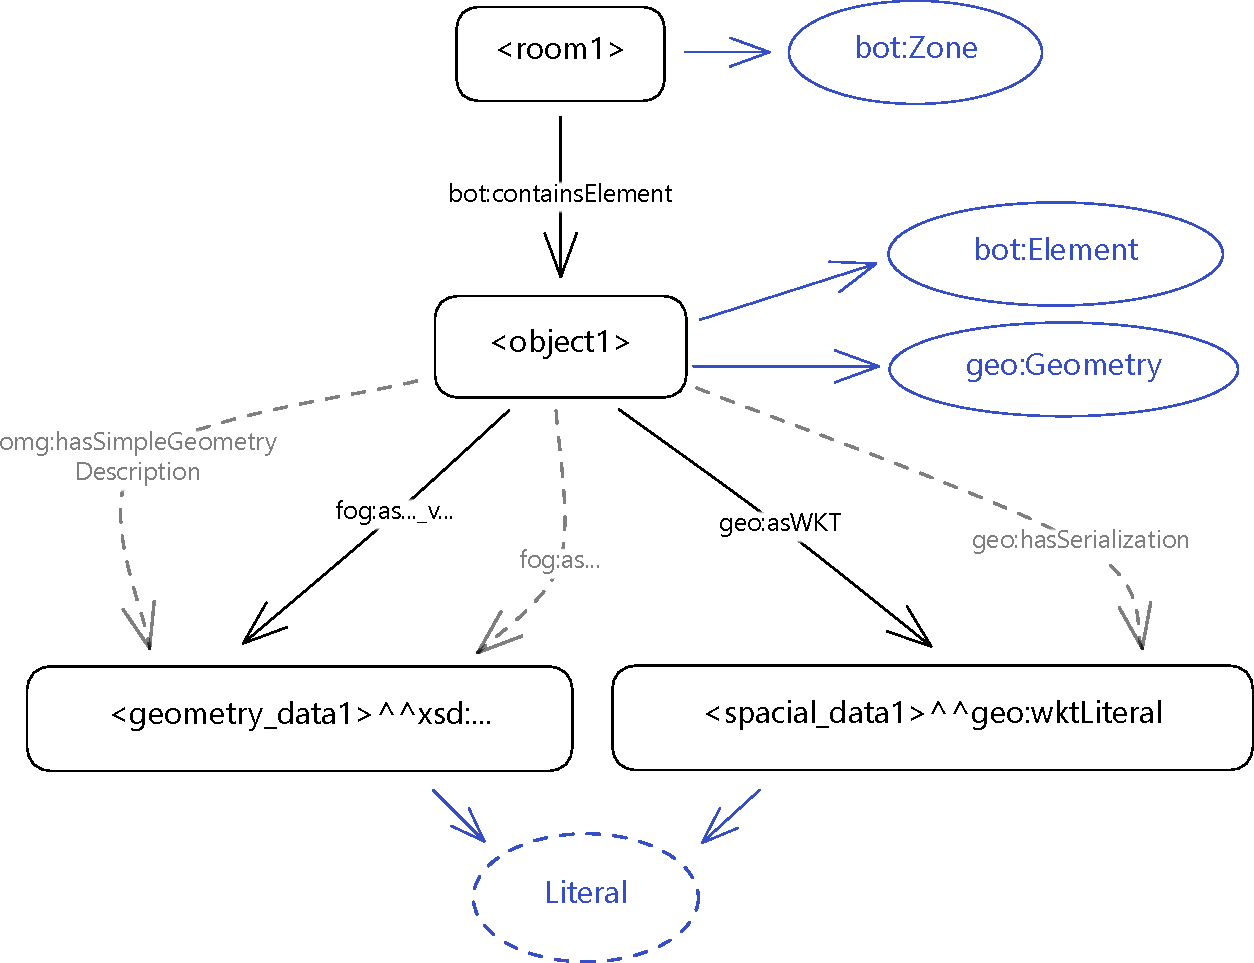
\includegraphics[width=0.8\textwidth]{figures/pdf/omg1.pdf}
    \caption[Serialization, \acs{omg} level 1]{Serialization of a geometry using the \acs{omg} level 1 pattern.}
    \label{fig:omg1}
\end{figure}


The separation into two sets allows for querying entities that have a \ac{wkt} serialization but are not located in a \mintinline{sparql}|bot:Space| (such as a floor, which would not be linked to a room) and entities that are located in a \mintinline{sparql}|bot:Space| that has a \ac{wkt} serialization. The latter variant uses the \mintinline{sparql}|bot:containsElement| or \mintinline{sparql}|bot:adjacentElement| properties to select entities within a room.

After filtering out spaces, the geometry of which is not needed by the viewer, it filters the entities' geometry based on a list of implemented/accepted formats by the receiving viewer. These last consist of a list of \ac{fog} super-properties inferred by their assignment. In other words: a triple in the \ac{rdf} graph of the form \mintinline{sparql}|?entity fog:asObj_v3.0| \mintinline{sparql}|?geometry_data| infers \mintinline{sparql}|?entity fog:asObj ?geometry_data| (as shown in Figure \ref{fig:omg1}). This allows for the use of a single property to query related formats while still permitting the declaration of more specific formats if needed.

In the end, the query returns a list of entities that are located in the same room as the observer, or are not located in a room but have a \ac{wkt} serialization that is validated by the GeoSPARQL filter function. Together with the needed metadata, which is further explained in Section \ref{sec:interactions}.

In the case of Listing \ref{lst:GeoSPARQLauto}, the GeoSPARQL \mintinline{sparql}|FILTER| uses the function \mintinline{sparql}|geof:sfWithin| to evaluate if the given point coordinates are within the \ac{wkt} serialization, which in most cases represents a \ac{wkt} polygon. For example:\\
\mintinline{turtle}|"POLYGON ((40 10, 30 10, 30 40, 40 40, 40 10))"^^geo:wktLiteral|

The use of GeoSPARQL results in a very efficient query, as the filtering is done directly in the query and does not require any post-processing. Although the lack of 3D capabilities is a limitation, it allows, in 2D to easily implement more complex algorithms leveraging the use of different functions. With which, together with a level 2 \ac{omg} pattern, \ac{lod} culling based on the distance to the observer can be implemented.

Selecting rooms and entities outside the room in which the observer is present is also conceivable when leveraging the use of the \mintinline{sparql}|bot:adjacentZone| property. Or using the GeoSPARQL distance to a room.
% query by distance, instance instead adjacent

\section{In viewer \enquote{bot:Space} identification} \label{sec:inViewer}
% - 1 database + 1 3D enabled instance (viewer) 
%   => viewer can raytrace identify wright space (little computation)
% - 2 layered viewer visible elements / invisible spaces
% - sequence diagram
%   - manual first step + adjacent spaces
%   - all spaces
%   - combination of spaces
% - sample queries
In this culling approach, ray tracing is employed to assess the room where the observer is situated. As illustrated in Figure \ref{fig:3participants}, out of the three participants, only one utilizes a 3D engine—a component capable of handling geometric modeling operations, such as ray tracing—referred to as the 3D viewer. In essence, both the \ac{sparql} endpoint and the external database lack the ability to perform 3D operations or evaluations. Consequently, this approach capitalizes on the 3D viewer to pinpoint the room in which the observer is positioned.

\begin{figure}[H]
    \centering
    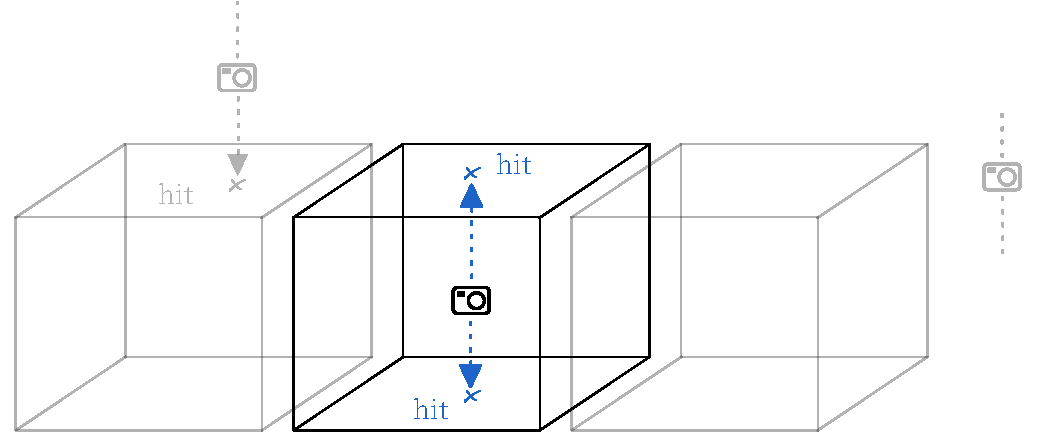
\includegraphics[width=0.8\textwidth]{figures/pdf/inViewer.pdf}
    \caption{In viewer \enquote{bot:Space} identification, with raytracing}
    \label{fig:raytrace}
\end{figure}

This process involves casting a ray from the observer's position both upwards and downwards, and evaluating the first intersection with a \mintinline{sparql}|bot:Space| entity. Unlike the previous approach, the geometry of the rooms themselves is required by the viewer, necessitating an initial query to load the rooms' geometry. By utilizing multiple layers in the viewer, the rooms' geometry can be concealed from the user while still being employed for ray tracing. Listing \ref{lst:findRoom} demonstrates the function used in this thesis prototype to assess the location. The scope of the picking is limited to the rooms using the cache's metadata, in this case \mintinline{ts}|lru: RefLRU|. Subsequently, two picking operations are carried out and compared, as depicted in Figure \ref{fig:raytrace}; if they match, the intersected room's \ac{uri} is returned.

\begin{listing}[h]
    \inputminted{ts}{dynamicQueries/inViewer/raytrace.ts}
    \vspace{-0.7cm}
    \caption{Typescript code for raytracing in viewer}
    \label{lst:findRoom}
\end{listing}

Once the room is identified, the query in Listing \ref{lst:BOTauto} is executed to retrieve the entities located within the room. This is achieved by querying the \mintinline{sparql}|bot:containsElement| property of the room. Similar to the previous method, it necessitates the combination of two sets of entities in this case: those located in the room and in the adjacent rooms themselves. This enables the optimization of the viewer by evaluating only the adjacent rooms, rather than all the rooms in the database.

The remainder of the query closely mirrors the previous one (Listing \ref{lst:GeoSPARQLauto}), with the distinction that it necessitates the additional storage of the \mintinline{sparql}|?botType| property to keep track of \ac{bot} classes and to identify \mintinline{sparql}|bot:Space| elements locally.

Due to the absence of \mintinline{sparql}|bot:adjacentZone| relations in the database used for the prototype, the query is unable to directly query the adjacent rooms. Instead, the property \mintinline{sparql}|bot:adjacentElement| is employed to query related room's adjacent walls and, consequently, the corresponding rooms. The lack of \ac{bot} relations in the utilized database was identified as a recurring issue in this thesis. Chapter \ref{ch:discussion} delves into this problem in greater detail.

This approach takes advantage of the 3D viewer and its engine to contribute to the culling process, although the first step requires downloading all the rooms' geometry. However, this step can be replaced by an initial manual localization by the user. By utilizing the adjacent rooms during subsequent queries, the impact on performance and resource usage remains minimal throughout the operation. In contrast to the \nameref{sec:inSituWKT}, this method is not limited to 2D but can be employed in 3D. However, it requires the geometry format of the room to be compatible with the viewer.

\begin{listing}[H]
    \inputminted{sparql}{dynamicQueries/inViewer/query.rq}
    \vspace{-0.7cm}
    \caption{Querying in viewer "bot:Space" identification}
    \label{lst:BOTauto}
\end{listing}

\section{In query OBJ geometry filtering} \label{sec:inQuery}
% - no geometric but string analysis in query
% - AABBox filtering of for example obj rooms
% - all negative points
This last approach is similar to the previous one, in that it also relies on the existing 3D geometry of the rooms, not their additional \ac{wkt} serialization. However, in contrast to \nameref{sec:inViewer}, the computation is once again offloaded to the \ac{sparql} endpoint. Since this endpoint is unable to perform geometric operations, a string analysis is performed instead.

The idea proposed by this thesis is to evaluate a string value, the literal representing the geometry, within a single \ac{sparql} query. As complicated string operations are difficult to perform with native \ac{sparql} functions, a custom JavaScript function is added to the \ac{sparql} endpoint. This function is then called within the query, as illustrated in Listing \ref{lst:OBJauto}. The prototype of this thesis uses GraphDB as its \ac{sparql} endpoint and \ac{rdf} database, which allows the addition of user-defined functions. Listing \ref{lst:graphdbNewFunction} demonstrates the addition of the function to the endpoint.

\begin{listing}[H]
    \inputminted{sparql}{dynamicQueries/inQuery/query.rq}
    \vspace{-0.7cm}
    \caption{Querying in query OBJ geometry filtering}
    \label{lst:OBJauto}
\end{listing}

The function itself (Listing \ref{lst:OBJautoFunction}) evaluates whether a given point is inside a geometry by extracting the vertex coordinates of the geometry literal to build an \ac{aabbox} in the form of a $3\times2$ matrix representing both a minimum and maximum value for each of the three axes. It then evaluates each point's coordinates against the given interval, returning a boolean value. The returned boolean can be interpreted by the \mintinline{sparql}|FILTER| clause inside the query, as illustrated in Listing \ref{lst:OBJauto}.

\begin{listing}[H]
    \inputminted{sparql}{dynamicQueries/inQuery/insert.rq}
    \vspace{-0.7cm}
    \caption{Inserting new javascript function in GraphDB}
    \label{lst:graphdbNewFunction}
\end{listing}

The advantages of this technique are that, similar to the previous proposal, 3D culling is achievable, there is no need for an extra serialization such as \ac{wkt}, and the computation is offloaded to the \ac{sparql} endpoint. However, the possibility to evaluate multiple geometry formats is on one side more flexible, as newer functions can interpret newer formats, not restricted by the viewer capabilities. This builds upon the concept of an all-knowing database serving a knowledge-free viewer (Section \ref{sec:proposal}). Although the possibility of allowing the JavaScript functions to fetch external files was not tested in this thesis, it could be a potential extension.

On the other hand, the function was tailored specifically for the \ac{sparql} endpoint used in this thesis, GraphDB, and would need to be adapted to other endpoints since no standard for user-defined functions was found during the research. Additionally, the JavaScript function was limited during the development of the prototype to a restricted scope of the JavaScript language, resembling the \ac{es5} version, which reduces the possibilities and optimization of the function.
\begin{listing}[H]
    \inputminted{js}{dynamicQueries/inQuery/function.js}
    \vspace{-0.7cm}
    \caption{Querying in situ WKT location}
    \label{lst:OBJautoFunction}
\end{listing}

